\documentclass[11pt,a4paper]{article}
\usepackage[margin=2.3cm]{geometry}
\usepackage{amsmath,amssymb,tikz,hyperref,lmodern}
\usepackage[T1]{fontenc}
\setlength{\parindent}{0pt}\setlength{\parskip}{6pt}
\newcommand{\code}[1]{\texttt{#1}}
\newcommand{\q}[2]{\medskip\noindent\textbf{Question #1 (#2 points).} }
\begin{document}
\begin{center}{\large CSC\_2F002\_EP --- Design and Analysis of Algorithms}\\[3pt]
{\Large\bfseries Practice Midterm --- Part I}\\[3pt]{\large Counting inversions}\end{center}
\textbf{Guidelines.} This part and Part II form one two-hour practice midterm, worth 20 points in total. Complete \code{inversions.py}; run \code{python3 test\_inversions.py} to test your functions. The tests are examples, not an exhaustive specification. Answer the exercise questions in Python comments at the indicated locations. Do not modify the input lists.

We wish to measure how far a list is from being sorted in nondecreasing order. An \emph{inversion} of a list \(A=[a_0,\ldots,a_{n-1}]\) is a pair of indices \((i,j)\) such that \(0\le i<j<n\) and \(a_i>a_j\). Equal values do not form an inversion. Entries can be negative or repeated. The inversion count of an empty list is zero.

For example, \code{A = [4, 1, 3, 1]} has four inversions: \((0,1), (0,2), (0,3), (2,3)\). The two occurrences of 1 are equal and do not form an inversion. A nondecreasing list has no inversions. For a strictly decreasing list of length \(n\), every pair of distinct indices is an inversion.
\begin{center}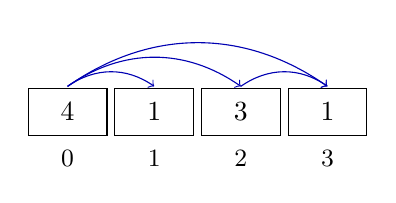
\begin{tikzpicture}[x=1.1cm,y=.65cm]
\foreach \x/\v in {0/4,1/1,2/3,3/1} {\node[draw,minimum width=1cm,minimum height=.6cm] at (\x,0) {\v}; \node at (\x,-.9) {\small\x};}
\draw[->,blue!70!black] (0,.5) to[bend left=35] (1,.5);
\draw[->,blue!70!black] (0,.5) to[bend left=35] (2,.5);
\draw[->,blue!70!black] (0,.5) to[bend left=35] (3,.5);
\draw[->,blue!70!black] (2,.5) to[bend left=35] (3,.5);
\end{tikzpicture}\\[4pt]\small Figure 1: Each arrow joins the indices of one inversion; indices appear below the cells.\end{center}
\q{1}{1} Complete \code{count\_after(A, i)}. Given a valid index \(i\), return the number of indices \(j>i\) for which \(a_i>a_j\). Its running time must be \(O(n)\). For example \code{count\_after([4,1,3,1], 2)} returns 1.

\q{2}{2} Complete \code{count\_naive(A)}. Return the total number of inversions of \(A\), using a direct examination of pairs. Its worst-case running time must be \(O(n^2)\). You may use \code{count\_after}. Test both functions before continuing.
\newpage
\textbf{A divide-and-conquer approach.} Let \(A=L+R\) where \(L\) is the left half and \(R\) the right half. Every inversion is either entirely in \(L\), entirely in \(R\), or crosses from \(L\) to \(R\). Assume that recursive calls return both the sorted values and the inversion count of each half. To finish, we must count crossing inversions and merge the two sorted halves.

Consider sorted lists \(L=[1,3,4]\) and \(R=[1,2,5]\). The entry 3 forms crossing inversions with 1 and 2, and so does 4. The crossing count is therefore 4. These pairs refer to occurrences, even if values are repeated. The sorted merge is \([1,1,2,3,4,5]\).

A merge can be performed with two indices \(i\) and \(j\), initially zero. Compare \(L[i]\) and \(R[j]\). If \(L[i]\le R[j]\), append \(L[i]\) and advance \(i\). Otherwise append \(R[j]\) and advance \(j\). Since \(L\) is sorted, in this second case \(R[j]\) is smaller than every element of \(L[i:]\). Hence it forms \(|L|-i\) crossing inversions. Finally append the unconsumed suffix, if any. On equality choose the entry of \(L\), since equal values do not count as inversions.

\begin{center}
\small\begin{tabular}{c|c|c|c}
Remaining \(L\)&Remaining \(R\)&Next action&New crossing inversions\\\hline
\([1,3,4]\)&\([1,2,5]\)&append left 1&0\\
\([3,4]\)&\([1,2,5]\)&append right 1&2\\
\([3,4]\)&\([2,5]\)&append right 2&2\\
\([3,4]\)&\([5]\)&append left 3, then left 4&0
\end{tabular}\\[6pt]\small Figure 2: The remaining 5 is appended after the left list is exhausted.
\end{center}
\q{3}{3} Complete \code{merge\_count(L, R)}. The input lists are already sorted in nondecreasing order. Return a tuple \code{(merged, count)}, where \code{merged} is a new sorted list containing all entries of \code{L} and \code{R}, including repetitions, and \code{count} is the number of crossing inversions. For example, the lists in Figure 2 return \code{([1,1,2,3,4,5], 4)}. Use the two-index merge above in \(O(|L|+|R|)\) time and \(O(|L|+|R|)\) output/auxiliary space. Do not mutate the input lists or use front deletion.
\newpage
\textbf{Putting the pieces together.} An inversion belongs to exactly one of the three categories: left, right, or crossing. Thus if the two recursive calls return counts \(c_L,c_R\) and the merge returns \(c_X\), the total is \(c_L+c_R+c_X\). The recursive result must also return the sorted list for use by its caller.

For \(A=[4,1,3,1]\), the left half \([4,1]\) has one inversion and sorts to \([1,4]\). The right half \([3,1]\) also has one inversion and sorts to \([1,3]\). Merging these sorted lists produces two additional crossing inversions, giving a total of four. The order of equal entries in the sorted result is irrelevant to the returned values, but they must not contribute to the crossing count.

\q{4}{3} Complete \code{sort\_and\_count(A)} using the divide-and-conquer scheme. Return \code{(sorted\_list, count)}. For an empty list or a singleton, return a new list with count zero. Split near the middle, make exactly one recursive call on each half and use \code{merge\_count}. The worst-case running time must be \(O(n\log n)\) for \(n\ge2\); do not call Python's sorting functions or the naive counting function. Python slicing is allowed for the two halves.

\q{5}{1} For \(n\) a power of two, suppose the running time satisfies \(T(1)=\Theta(1)\) and \(T(n)=2T(n/2)+\Theta(n)\). In the comment block marked \code{Q5} in \code{inversions.py}, give a brief justification of the asymptotic bound for \(T(n)\). You may use a recursion tree or the master theorem; state why its assumptions match the algorithm.

\textbf{Additional checks.} The result for \code{[2,2,2]} is zero; for \code{[3,2,1]} it is three. A list may contain many equal values across the split, so using \(\le\) rather than \(<\) in the left-choice case matters. The returned sorted list must preserve the multiplicity of every value.
\end{document}
